\chapter{PENGUJIAN DAN EVALUASI}

\section{Lingkungan Uji Coba}
	Lingkungan pengujian menggunakan komponen-komponen yang terdiri dari: satu \textit{server publisher}, satu \textit{server publish/subscribe}, satu \textit{server aplikasi}, satu \textit{server API}, satu \textit{server database}, satu agen SNMP dan satu komputer penguji. Semua \textit{server} menggunakan vitual machine yang dipasang pada \textit{Hypervisor} Proxmox. Lalu, untuk komputer penguji menggunakan satu buah laptop sebagai klien yang digunakan untuk menerima data yang dikirim oleh publisher dan melakukan skenario pengetesan pada REST API. Pengujian dilakukan di Laboratoriom Arsitektur dan Jaringan Komputer Jurusan Teknik Informatika ITS. \\
    \indent Spesifikasi untuk setiap komponen yang digunakan ditunjukkan pada Tabel \ref{spesifikasikomponen}.
    \begin{longtable}{|p{0.05\textwidth}|p{0.18\textwidth}|p{0.33\textwidth}|p{0.33\textwidth}|}					\caption{Spesifikasi Komponen} \label{spesifikasikomponen} \\
        \hline
        \textbf{No} & \textbf{Komponen} & \textbf{Perangkat Keras} & \textbf{Perangkat Lunak} \\ \hline
        \endfirsthead
        \caption[]{Spesifikasi Komponen} \\
        \hline
        \textbf{No} & \textbf{Komponen} & \textbf{Perangkat Keras} & \textbf{Perangkat Lunak} \\ \hline
        \endhead
        \endfoot
        \endlastfoot

    	1 & Publisher & 1 core processor, 512 MB RAM, 20GB HDD pada virtualisasi Proxmox & Ubuntu 16.04 LTS, Python2.7, Nagios \\ \hline
        2 & Pub/Sub & 1 core processor, 512 MB RAM, 20GB HDD pada virtualisasi Proxmox & Ubuntu 16.04 LTS, RabbitMQ \\ \hline
        3 & Application & 1 core processor, 512 MB RAM, 20GB HDD pada virtualisasi Proxmox & Ubuntu 16.04 LTS, Node.JS, Python 2.7 \\ \hline
        4 & REST API & 1 core processor, 512 MB RAM, 20GB HDD pada virtualisasi Proxmox & Ubuntu 16.04 LTS, Docker 17.03.0-ce, Python 2.7 \\ \hline
        5 & Database & 1 core processor, 512 MB RAM, 20GB HDD pada virtualisasi Proxmox & Ubuntu 16.04 LTS, MySQL Server \\ \hline
        6 & Agen SNMP & Mikrotik Routerboard Cloud Switch Series & Agen SNMP \\ \hline
        7 & Komputer penguji & Processor Intel i5-3210M, 8 GB RAM & Ubuntu 16.04 LTS, JMeter 4.0 \\ \hline
    \end{longtable}
    
    \indent Untuk akses ke masing-masing komponen, digunakan IP private yang disediakan untuk masing-masing komponen tersebut. Detailnya ditunjukkan pada Tabel \ref{ipdomainserver}.
    			\begin{longtable}{|p{0.05\textwidth}|p{0.33\textwidth}|p{0.44\textwidth}|}					\caption{IP dan Domain Server} \label{ipdomainserver} \\
					\hline
					\textbf{No} & \textbf{Server} & \textbf{IP dan Domain} \\ \hline
					\endfirsthead
					\caption[]{IP dan Domain Server} \\
					\hline
					\textbf{No} & \textbf{Server} & \textbf{IP dan Domain} \\ \hline
					\endhead
					\endfoot
					\endlastfoot
					
                    1 & Publisher & 10.151.36.97 \\ \hline
                    2 & Pub/Sub & 10.151.36.98 \\ \hline
                    3 & Application & 10.151.36.99 \\ \hline
                    4 & REST API & 10.151.36.100 \\ \hline
                    5 & Database & 10.151.36.101 \\ \hline
                    6 & Agen SNMP & 10.151.36.3 \\ \hline
                    7 & Komputer Penguji & 10.151.36.153 \\ \hline
				\end{longtable}
    
\section{Skenario Uji Coba} \label{skenarioujicoba}
	Uji coba akan dilakukan untuk mengetahui keberhasilan sistem yang telah dibangun. Skenario pengujian dibedakan menjadi 2 bagian, yaitu:
    \begin{itemize}
    \item \textbf{Uji Fungsionalitas} \\
    	Pengujian ini didasarkan pada fungsionalitas yang disajikan sistem.
    \item \textbf{Uji Performa} \\
    	Pengujian ini untuk menguji kecepatan respon sistem terhadap sejumlah permintaan ke aplikasi secara bersamaan. Pengujian dilakukan dengan melakukan \textit{benchmark} pada sistem.
    \end{itemize}
    
    \subsection{Skenario Uji Coba Fungsionalitas}
    	Uji fungsionalitas dibagi menjadi 2, yaitu uji fungsionalitas antarmuka aplikasi dan uji fungsionalitas endpoint REST API.
        
        \subsubsection{Uji Fungsionalitas Antarmuka Aplikasi} \label{ujifungsionalitasantarmuka}
        	Pengujuian ini dilakukan untuk memeriksa apakah semua fungsi yang berada pada aplikasi dapat dijalankan dengan benar. Pengujian dilakukan dengan cara mengakses antarmuka yang berhubungan dengan tugas akhir ini lalu menjalankan fitur yang disediakan pada tiap-tiap antarmuka.
        	
        	Rancangan pengujian dan hasil yang diharapkan dapat dilihat pada tabel \ref{ujiaplikasi}.
        	
            \begin{longtable}{|p{0.05\textwidth}|p{0.20\textwidth}|p{0.30\textwidth}|p{0.27\textwidth}|}					\caption{Skenario Uji Fungsionalitas Antarmuka Aplikasi} \label{ujiaplikasi} \\
					\hline
					\textbf{No} & \textbf{Fitur} & \textbf{Uji Coba} & \textbf{Hasil Harapan} \\ \hline
					\endfirsthead
					\caption[]{Skenario Uji Fungsionalitas Antarmuka Aplikasi} \\
					\hline
					\textbf{No} & \textbf{Fitur} & \textbf{Uji Coba} & \textbf{Hasil Harapan} \\ \hline
					\endhead
					\endfoot
					\endlastfoot
					
                    1 & Autentikasi pengguna untuk masuk kedalam sistem. & Pengguna memasukkan username dan password masing-masing milik pengguna pada form yang telah disediakan. & Pengguna dapat masuk ke halaman utama aplikasi setelah menekan tombol "login"\\ \hline
                    2 & Menampilkan seluruh data perangkat. & Pengguna menekan \textit{menu} "DEVICE MANAGEMENT" pada \textit{sidebar}. & Sistem menampilkan seluruh data perangkat yang terdaftar pada sistem. data yang ditampilkan meliputi: nama perangkat, tipe perangkat, alamat perangkat dan lokasi perangkat. serta terdapat tombol informasi untuk melihat data masing-masing perangkat secara rinci dan tombol hapus untuk menghapus data perangkat yang terdaftar pada sistem. \\ \hline
                    3 & Menampilkan rincian data perangkat & Pengguna menekan tombol informasi yang tersedia pada tabel pada halaman menampilkan seluruh data perangkat. & Sistem menampilkan data perangkat terkait secara rinci. data yang ditampilkan meliputi: profil perangkat, pelanggan dari perangkat dan OID (Informasi yang disediakan pada perangkat terkait). \\ \hline
                    4 & Menghapus data perangkat. & Pengguna menekan tombol hapus yang tersedia pada tabel pada halaman menampilkan seluruh data perangkat. & Sistem menghapus data perangkat terkait secara permanen. \\ \hline
					5 & Menyunting data perangkat. & Pengguna menekan tombol ubah data pada halaman rincian data perangkat lalu mengubah data yang tersedia pada form yang berisi data sebelumnya. & Sistem mengubah data yang lama dengan data yang baru dimasukkan oleh pengguna. \\ \hline
                    6 & Berlangganan Data Perangkat. & Pengguna menekan tombol "Subscribe" yang tersedia pada halaman rincian data perangkat. & Sistem menandai bahwa perangkat atau OID (Informasi pada perangkat) yang terkait telat dilanggani. tombol akan berubah menjadi "Unsubscribe"\\ \hline
                    7 & Memantau kondisi perangkat yang telah dilanggani. & Pengguna menekan \textit{menu} "MONITOR" pada \textit{sidebar}. & Sistem menampilkan kondisi dari seluruh perangkat yang telah dilanggani informasinya oleh pengguna. \\ \hline
				\end{longtable}
            
        \subsubsection{Uji Fungsionalitas Endpoint REST API}\label{ujifungsionalitasrestapi}
        	Pengujian ini dilakukan untuk memeriksa apakah seluruh fungsi dan \textit{endpoint} yang berhubungan dengan tugas akhir ini dan tersedia pada sistem dapat bekerja dengan semestinya. Pengujian dilakukan dengan cara mengakses \textit{endpoint} dengan metode tertentu disertai dengan \textit{header} autentikasi JWT . Rancangan pengujian dan hasil yang diharapkan ditunjukkan dengan Tabel \ref{ujirestapi}.
            
            \begin{longtable}{|p{0.05\textwidth}|p{0.20\textwidth}|p{0.30\textwidth}|p{0.27\textwidth}|}					\caption{Skenario Uji Fungsionalitas REST API} \label{ujirestapi} \\
            	\hline
            	\textbf{No} & \textbf{\textit{Endpoint}} & \textbf{Uji Coba} & \textbf{Hasil Harapan} \\ \hline
            	\endfirsthead
            	\caption[]{Skenario Uji Fungsionalitas REST API} \\
            	\hline
            	\textbf{No} & \textbf{\textit{Endpoint}} & \textbf{Uji Coba} & \textbf{Hasil Harapan} \\ \hline
            	\endhead
            	\endfoot
            	\endlastfoot
            	
            	1 & /login. & Mengakses endpoint dengan header autentikasi JWT dan metode POST, disertai dengan body bertipe JSON yang dilengkapi dengan beberapa parameter seperti: username dan password. & REST API mengembalikan respon berupa pesan berhasil dan token JWT jika berhasil, lalu mengembalikan pesan gagal jika gagal. \\ \hline
            	2 & /devices. & Mengakses endpoint dengan header autentikasi JWT dan metode GET. & jika berhasil, REST API mengembalikan respon berupa seluruh data yang tersedia pada sistem dalam bentuk json. tiap datanya meliputi: nama perangkat, tipe perangkat, alamat perangkat dan lokasi perangkat. Jika terjadi kegagalan, REST API akan mengembalikan pesan gagal. \\ \hline
            	3 & /devices/ <string:id> & Mengakses endpoint dengan header autentikasi JWT, metode GET dan menyertakan ID perangkat pada endpoint. & jika berhasil, REST API mengembalikan respon berupa seluruh data yang tersedia pada sistem dalam bentuk json. tiap datanya meliputi: nama perangkat, tipe perangkat, alamat perangkat, lokasi perangkat, subscriber perangkat dan OID (informasi yang tersedia pada perangkat). Jika terjadi kegagalan, REST API akan mengembalikan pesan gagal. \\ \hline
            	4 & /devices /create. & Mengakses endpoint dengan header autentikasi JWT dan metode POST, disertai dengan body bertipe JSON yang dilengkapi dengan beberapa parameter seperti: \textit{name}, \textit{type}, \textit{address} dan \textit{location} & jika berhasil, REST API mengembalikan respon berupa pesan berhasil. Jika gagal, maka REST API akan mengambalikan pesan gagal. \\ \hline
            	5 & /devices /edit /<string:id> & Mengakses endpoint dengan header autentikasi JWT, metode POST, menyertakan ID perangkat pada endpoint dan disertai dengan body bertipe JSON yang dilengkapi dengan beberapa parameter seperti: \textit{name}, \textit{type}, \textit{address} dan \textit{location}. & jika berhasil, REST API mengembalikan respon berupa pesan berhasil. Jika gagal, maka REST API akan mengambalikan pesan gagal. \\ \hline
            	6 & /devices /delete & Mengakses endpoint dengan header autentikasi JWT dan metode DELETE, disertai dengan body bertipe JSON yang dilengkapi dengan parameter ID perangkat. & jika berhasil, REST API mengembalikan respon berupa pesan berhasil. Jika gagal, maka REST API akan mengambalikan pesan gagal. \\ \hline
            	7 & /oid /create & Mengakses endpoint dengan header autentikasi JWT dan metode POST, disertai dengan body bertipe JSON yang dilengkapi dengan beberapa parameter seperti: oidname, oid dan devices\_id & jika berhasil, REST API mengembalikan respon berupa pesan berhasil. Jika gagal, maka REST API akan mengambalikan pesan gagal. \\ \hline
            	8 & /oid /edit & Mengakses endpoint dengan header autentikasi JWT dan metode POST, disertai dengan body bertipe JSON yang dilengkapi dengan beberapa parameter seperti: oidname, oid dan devices\_id & jika berhasil, REST API mengembalikan respon berupa pesan berhasil. Jika gagal, maka REST API akan mengambalikan pesan gagal. \\ \hline
            	9 & /oid /delete & Mengakses endpoint dengan header autentikasi JWT dan metode POST, disertai dengan body bertipe JSON yang dilengkapi dengan parameter parameter ID perangkat. & jika berhasil, REST API mengembalikan respon berupa pesan berhasil. Jika gagal, maka REST API akan mengambalikan pesan gagal. \\ \hline
            	10 & /subscribe /devices & Mengakses endpoint dengan header autentikasi JWT dan metode POST, disertai dengan body bertipe JSON yang dilengkapi dengan beberapa parameter seperti: device\_id dan users\_id. & jika berhasil, REST API mengembalikan respon berupa pesan berhasil. Jika gagal, maka REST API akan mengambalikan pesan gagal. \\ \hline
            	11 & /unsubscribe /devices & Mengakses endpoint dengan header autentikasi JWT dan metode POST, disertai dengan body bertipe JSON yang dilengkapi dengan beberapa parameter seperti: device\_id dan users\_id. & jika berhasil, REST API mengembalikan respon berupa pesan berhasil. Jika gagal, maka REST API akan mengambalikan pesan gagal. \\ \hline
            	12 & /subscribe /oid & Mengakses endpoint dengan header autentikasi JWT dan metode POST, disertai dengan body bertipe JSON yang dilengkapi dengan beberapa parameter seperti: oid\_id dan users\_id. & jika berhasil, REST API mengembalikan respon berupa pesan berhasil. Jika gagal, maka REST API akan mengambalikan pesan gagal. \\ \hline
            	13 & /unsubscribe /oid & Mengakses endpoint dengan header autentikasi JWT dan metode POST, disertai dengan body bertipe JSON yang dilengkapi dengan beberapa parameter seperti: oid\_id dan users\_id. & jika berhasil, REST API mengembalikan respon berupa pesan berhasil. Jika gagal, maka REST API akan mengambalikan pesan gagal. \\ \hline
            \end{longtable}
            
        
    \subsection{Skenario Uji Coba Performa}
    	Uji performa dilakukan dengan dua langkah, yaitu uji performa REST api dan uji performa publish/subscribe. Arsitektur sistem yang dirancang untuk pengujian dapat dilihat pada gambar \ref{arsitekturpengujian}.
    	
    	Uji coba REST API dilakukan dengan menggunakan satu buah laptop untuk melakukan akses secara bersamaan ke REST API menggunakan aplikasi JMeter. Laptop akan mencoba mengaskses REST API yang sudah berjalan pada suatu server, dengan alamat IP 10.151.36.100.
    	
    	Uji performa selanjutnya yaitu uji performa publish/subscribe dilakukan dengan cara menghitung waktu pengiriman. pengiriman dilakukan dari publisher yang berada pada server dengan alamat IP 10.151.36.97 menuju consumer yang berada pada alamat IP 10.151.36.99.
    	
    	\begin{figure}[H]
    		\centering
    		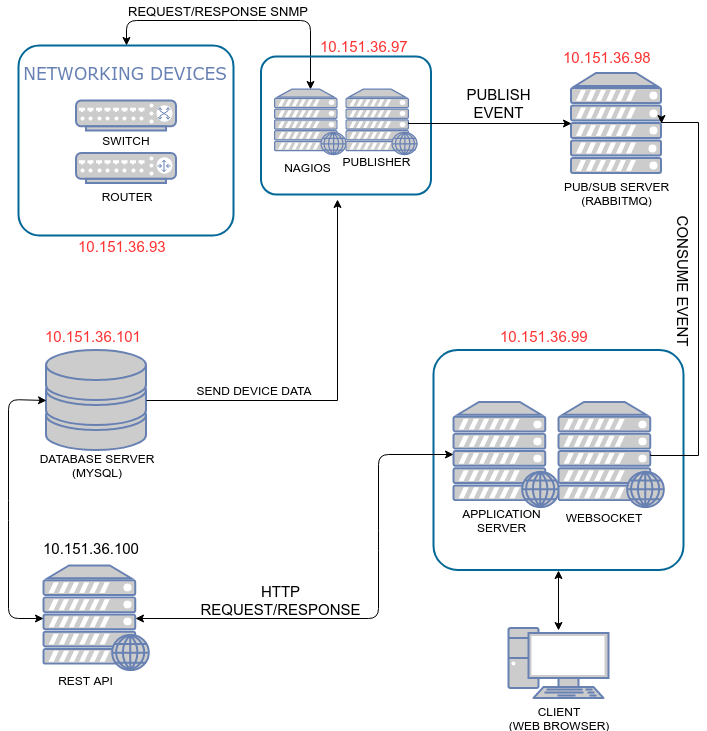
\includegraphics[width=9cm]{Images/C-5/arsitesting.png}
    		\caption{Arsitektur Sistem yang Digunakan Untuk Pengujian}
    		\label{arsitekturpengujian}
    	\end{figure}
        
    	\subsubsection{Uji Performa Kecepatan REST API Menangani \textit{Request}}
        	Pengujian dilakukan dengan mengukur jumlah waktu yang diperlukan oleh REST API untuk menyelesaikan \textit{request} yang dilakukan oleh komputer penguji. Waktu yang diukur adalah perbedaan jarak antara \textit{request} pertama dan terakhir dilakukan oleh klien yang mendapatkan balasan dari \textit{server}.
        	
        	Percobaan dilakukan dengan membuat thread untuk setiap akses ke REST API. Pengujian akan berlangsung bertahap mulai dari 300, 600, 900, 1200 dan 1500 thread dengan pengulangan 5 kali untuk setiap \textit{event}. Dari hasil pengujian akan didapatkan waktu respon terhadap permintaan. Waktu tersebut digunakan untuk membuat grafik kesimpulan.
        \subsubsection{Uji Performa Kecepatan Pengiriman Data Dari Publisher Menuju Consumer}
        	Pengujian dilakukan dengan menghitung waktu yang diperlukan publisher untuk mengirimkan data hingga sampai kepada consumer melalui pub/sub server. Pengujian dilakukan dengan cara mengurangi waktu (timestamp) yang dideklarasikan saat publisher mengirimkan data dengan waktu (timestamp) saat pesan sampai di consumer dan siap untuk dikirimkan kepada client melalu websocket.
    
\section{Hasil Uji Coba dan Evaluasi}
	Berikut dijelaskan hasil uji coba dan evaluasi berdasarkan skenario yang telah dijelaskan pada subbab \ref{skenarioujicoba}.
    
	\subsection{Uji Fungsionalitas}
    	Berikut dijelaskan hasil pengujian fungsionalitas pada sistem yang dibangun.
        
        \subsubsection{Uji Fungsionalitas Antarmuka Aplikasi}
    	Pengujian dilakukan sesuai dengan skenario yang dijelaskan pada subbab \ref{ujifungsionalitasantarmuka} dan pada Tabel \ref{ujiaplikasi}. Hasil pengujian seperti tertera pada Tabel \ref{hasilujicobaaplikasi}.
        
        \begin{longtable}{|p{0.05\textwidth}|p{0.55\textwidth}|p{0.22\textwidth}|}					\caption{Hasil Uji Coba Mengelola Aplikasi Berbasis Docker} \label{hasilujicobaaplikasi} \\
					\hline
					\textbf{No} & \textbf{Uji Coba} & \textbf{Hasil} \\ \hline
					\endfirsthead
					\caption[]{Hasil Uji Coba Mengelola Aplikasi Berbasis Docker} \\
					\hline
					\textbf{No} & \textbf{Uji Coba} & \textbf{Hasil} \\ \hline
					\endhead
					\endfoot
					\endlastfoot
					
                    1 & Pengguna memasukkan username dan password masing-masing milik pengguna pada form yang telah disediakan. & Sukses \\ \hline
                    2 & Pengguna menekan \textit{menu} "DEVICE MANAGEMENT" pada \textit{sidebar}. & Sukses \\ \hline
                    3 & Pengguna menekan tombol informasi yang tersedia pada tabel pada halaman menampilkan seluruh data perangkat. & Sukses \\ \hline
                    4 & Pengguna menekan tombol hapus yang tersedia pada tabel pada halaman menampilkan seluruh data perangkat. & Sukses \\ \hline
					5 & Pengguna menekan tombol ubah data pada halaman rincian data perangkat lalu mengubah data yang tersedia pada form yang berisi data sebelumnya. & Sukses \\ \hline
                    6 & Pengguna menekan tombol "Subscribe" yang tersedia pada halaman rincian data perangkat. & Sukses \\ \hline
					7 & Pengguna menekan \textit{menu} "MONITOR" pada \textit{sidebar}. & Sukses \\ \hline
				\end{longtable}
    		Sesuai dengan skenario uji coba  yang diberikan pada Tabel \ref{ujiaplikasi}, hasil uji coba menunjukkan semua skenario berhasil ditangani.
        
    	\subsubsection{Uji Fungsionalitas Endpoint REST API}
        	Pengujian dilakukan sesuai dengan skenario yang dijelaskan pada subbab \ref{ujifungsionalitasrestapi} dan pada Tabel \ref{ujirestapi}. Hasil pengujian seperti tertera pada Tabel \ref{hasilujirestapi}.
        	
        		\begin{longtable}{|p{0.05\textwidth}|p{0.20\textwidth}|p{0.30\textwidth}|p{0.27\textwidth}|}					\caption{Skenario Uji Fungsionalitas REST API} \label{hasilujirestapi} \\
        			\hline
        			\textbf{No} & \textbf{\textit{Endpoint}} & \textbf{Uji Coba} & \textbf{Hasil Harapan} \\ \hline
        			\endfirsthead
        			\caption[]{Skenario Uji Fungsionalitas REST API} \\
        			\hline
        			\textbf{No} & \textbf{\textit{Endpoint}} & \textbf{Uji Coba} & \textbf{Hasil} \\ \hline
        			\endhead
        			\endfoot
        			\endlastfoot
        			
        			1 & /login. & Mengakses endpoint dengan header autentikasi JWT dan metode POST, disertai dengan body bertipe JSON yang dilengkapi dengan beberapa parameter seperti: username dan password. & OK - REST API mengembalikan respon berupa pesan berhasil \\ \hline
        			2 & /devices. & Mengakses endpoint dengan header autentikasi JWT dan metode GET. & OK - REST API mengembalikan respon berupa seluruh data yang tersedia pada sistem dalam bentuk json. tiap datanya meliputi: nama perangkat, tipe perangkat, alamat perangkat dan lokasi perangkat. \\ \hline
        			3 & /devices/ <string:id> & Mengakses endpoint dengan header autentikasi JWT, metode GET dan menyertakan ID perangkat pada endpoint. & OK - REST API mengembalikan respon berupa seluruh data yang tersedia pada sistem dalam bentuk json. tiap datanya meliputi: nama perangkat, tipe perangkat, alamat perangkat, lokasi perangkat, subscriber perangkat dan OID (informasi yang tersedia pada perangkat). \\ \hline
        			4 & /devices /create. & Mengakses endpoint dengan header autentikasi JWT dan metode POST, disertai dengan body bertipe JSON yang dilengkapi dengan beberapa parameter seperti: \textit{name}, \textit{type}, \textit{address} dan \textit{location} & OK - REST API mengembalikan respon berupa pesan berhasil. \\ \hline
        			5 & /devices /edit /<string:id> & Mengakses endpoint dengan header autentikasi JWT, metode POST, menyertakan ID perangkat pada endpoint dan disertai dengan body bertipe JSON yang dilengkapi dengan beberapa parameter seperti: \textit{name}, \textit{type}, \textit{address} dan \textit{location}. & OK - REST API mengembalikan respon berupa pesan berhasil. \\ \hline
        			6 & /devices /delete & Mengakses endpoint dengan header autentikasi JWT dan metode DELETE, disertai dengan body bertipe JSON yang dilengkapi dengan parameter ID perangkat. & OK - REST API mengembalikan respon berupa pesan berhasil. \\ \hline
        			7 & /oid /create & Mengakses endpoint dengan header autentikasi JWT dan metode POST, disertai dengan body bertipe JSON yang dilengkapi dengan beberapa parameter seperti: oidname, oid dan devices\_id & OK - REST API mengembalikan respon berupa pesan berhasil. \\ \hline
        			8 & /oid /edit & Mengakses endpoint dengan header autentikasi JWT dan metode POST, disertai dengan body bertipe JSON yang dilengkapi dengan beberapa parameter seperti: oidname, oid dan devices\_id & OK - REST API mengembalikan respon berupa pesan berhasil. \\ \hline
        			9 & /oid /delete & Mengakses endpoint dengan header autentikasi JWT dan metode POST, disertai dengan body bertipe JSON yang dilengkapi dengan parameter parameter ID perangkat. & OK - REST API mengembalikan respon berupa pesan berhasil. \\ \hline
        			10 & /subscribe /devices & Mengakses endpoint dengan header autentikasi JWT dan metode POST, disertai dengan body bertipe JSON yang dilengkapi dengan beberapa parameter seperti: device\_id dan users\_id. & OK - REST API mengembalikan respon berupa pesan berhasil. \\ \hline
        			11 & /unsubscribe /devices & Mengakses endpoint dengan header autentikasi JWT dan metode POST, disertai dengan body bertipe JSON yang dilengkapi dengan beberapa parameter seperti: device\_id dan users\_id. & OK - REST API mengembalikan respon berupa pesan berhasil. \\ \hline
        			12 & /subscribe /oid & Mengakses endpoint dengan header autentikasi JWT dan metode POST, disertai dengan body bertipe JSON yang dilengkapi dengan beberapa parameter seperti: oid\_id dan users\_id. & OK - REST API mengembalikan respon berupa pesan berhasil. \\ \hline
        			13 & /unsubscribe /oid & Mengakses endpoint dengan header autentikasi JWT dan metode POST, disertai dengan body bertipe JSON yang dilengkapi dengan beberapa parameter seperti: oid\_id dan users\_id. & OK - REST API mengembalikan respon berupa pesan berhasil. \\ \hline
        		\end{longtable}
    \pagebreak
    \subsection{Hasil Uji Performa}
    	Seperti yang sudah dijelaskan pada subbab \ref{skenarioujicoba} pengujian performa dilakukan dengan menghitung respon dari sistem terhadap sejumlah permintaan (\textit{request}) secara bersamaan.
        \begin{longtable}{|p{0.33\textwidth}|p{0.35\textwidth}|}
        \caption{Jumlah \textit{Request} ke Aplikasi} \label{trequest} \\
            \hline
            \textbf{\textit{Concurrent Users}} & \textbf{Jumlah \textit{Request}} \\ \hline
            \endfirsthead
            \caption[]{Jumlah \textit{Request} ke Aplikasi} \\
            \hline
            \textbf{\textit{Concurrent Users}} & \textbf{Jumlah \textit{Request}} \\ \hline
            \endhead
            \endfoot
            \endlastfoot
            
            800 & $\pm$ 16.925 \\ \hline
            1.600 & $\pm$ 26.650 \\ \hline
            2.400 & $\pm$ 34.943 \\ \hline
            3.200 & $\pm$ 50.092 \\ \hline
            4.000 & $\pm$ 57.750 \\ \hline
					
		\end{longtable}
        
        Pada Tabel \ref{tjumlahcontainer} dapat dilihat jumlah \textit{container} yang terbentuk selama proses \textit{request} dari \textit{user} yang dilakukan selama enam kali. Nilai yang ditampilkan berupa nilai rata-rata selama percobaan dibulatkan ke atas. Sistem dapat menyediakan \textit{container} sesuai dengan jumlah \textit{request} yang diberikan, semakin banyak \textit{request} yang dilakukan, maka \textit{container} yang disediakan akan semakin banyak. Nilai \textit{container} tersebut didapatkan dari perhitungan \textit{proactive model}. Selain melihat jumlah \textit{request}, penentuan \textit{container} yang dibentuk juga dari jumlah sumber daya yang digunakan \textit{container} berdasarkan perhitungan menggunakan \textit{reactive model}. Pada Gambar \ref{gjumlahcontainer} dapat dilihat grafik dari jumlah \textit{container} yang terbentuk berdasarkan jumlah \textit{request} yang dilakukan.
        
        \begin{longtable}{|p{0.25\textwidth}|p{0.20\textwidth}|p{0.20\textwidth}|}
        \caption{Jumlah \textit{Container}} \label{tjumlahcontainer} \\
            \hline
            \textbf{\textit{Concurrent Users}} & \textbf{Maksimal \textit{Container}} &  \textbf{Rata-rata \textit{Container}} \\ \hline
            \endfirsthead
            \caption[]{Jumlah \textit{Container}} \\
            \hline
            \textbf{\textit{Concurrent Users}} & \textbf{Maksimal \textit{Container}} &  \textbf{Rata-rata \textit{Container}} \\ \hline
            \endhead
            \endfoot
            \endlastfoot
            
            800 & 6 & 2 \\ \hline
            1.600 & 8 & 3 \\ \hline
            2.400 & 14 & 6 \\ \hline
            3.200 & 18 & 7 \\ \hline
            4.000 & 30 & 11 \\ \hline
					
		\end{longtable}
        
        \begin{figure}[H]
				\centering
				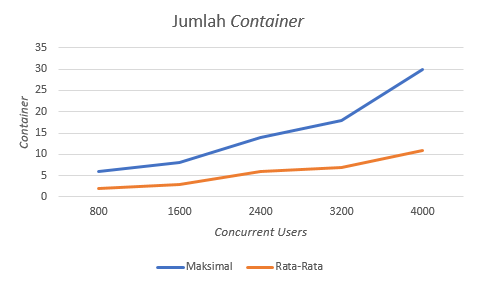
\includegraphics[width=8.7cm,height=4.7cm]{Images/C-5/jumlahcontainer.png}
				\caption{Grafik Jumlah \textit{Container}}
				\label{gjumlahcontainer}
			\end{figure}
        
    	\subsubsection{Kecepatan Menangani \textit{Request}}
        	Dari hasil uji coba kecepatan menangani \textit{request}, dapat dilihat pada Table \ref{kecepatanrequest} dalam satuan detik bahwa semakin banyak \textit{concurrent users}, semakin lama pula waktu yang diperlukan untuk menyeselaikannya. Request paling cepat ditangani dengan menggunakan prediksi ARIMA(4,1,0) dan paling lambat menggunakan ARIMA(1,1,0). Hal tersebut terjadi karena kurang bagusnya hasil prediksi yang dihasilkan oleh ARIMA(1,1,0) yang mana kadang hasil prediksinya terlalu rendah atau terlalu tinggi.
            Dari hasil percobaan tersebut, dapat dilihat bahwa hampir semua \textit{request} dapat ditangani di bawah satu menit. Lalu grafik hasil uji coba perhitungan kecepatan menangani \textit{request} ditunjukkan pada Gambar \ref{grunningtime}.
            \begin{longtable}{|p{0.22\textwidth}|p{0.10\textwidth}|p{0.10\textwidth}|p{0.10\textwidth}|p{0.10\textwidth}|p{0.10\textwidth}|}
        \caption{Kecepatan Menangani \textit{Request}} \label{kecepatanrequest} \\
            \hline
            & \textbf{800} & \textbf{1600} & \textbf{2400} & \textbf{3200} & \textbf{4000} \\ \hline
            \endfirsthead
            \caption[]{Kecepatan Menangani \textit{Request}} \\
            \hline
            & \textbf{800} & \textbf{1600} & \textbf{2400} & \textbf{3200} & \textbf{4000} \\ \hline
            \endhead
            \endfoot
            \endlastfoot
			
          	ARIMA(1,1,0) & 34.167 & 43.286 & 48.143 & 63.857 & 62.286 \\ \hline
            ARIMA(2,1,0) & 27.429 & 38.571 & 44.143 & 42.143 & 57.857 \\ \hline
            ARIMA(3,1,0) & 32.429 & 36.000 & 38.429 & 41.571 & 43.857 \\ \hline
            ARIMA(4,1,0) & 24.857 & 31.571 & 34.429 & 42.143 & 52.714 \\ \hline
		\end{longtable}
         
        	\begin{figure}[H]
				\centering
				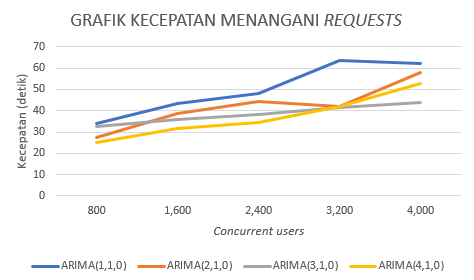
\includegraphics[width=8.7cm,height=4.7cm]{Images/C-5/runningtime.png}
				\caption{Grafik Kecepatan Menangani \textit{Request}}
				\label{grunningtime}
			\end{figure}
            
        \subsubsection{Penggunaan CPU}
        	Dari hasil uji coba penggunaan CPU pada \textit{server master host}, penggunaan CPU berada di bawah 15\%. Penggunaan CPU yang diukur adalah penggunaan CPU yang dilakukan oleh \textit{container} dari aplikasi, tidak termasuk sistem. Jumlah \textit{core} yang dimiliki oleh \textit{processor} di \textit{server master host} adalah 8 buah, yang artinya kurang lebih hanya satu core yang digunakan untuk menangani semua \textit{request}. Hasil pengukuran penggunaan CPU dapat dilihat pada Tabel \ref{penggunaancpu}
            
            \begin{longtable}{|p{0.22\textwidth}|p{0.10\textwidth}|p{0.10\textwidth}|p{0.10\textwidth}|p{0.10\textwidth}|p{0.10\textwidth}|}
        \caption{Penggunaan CPU} \label{penggunaancpu} \\
            \hline
            & \textbf{800} & \textbf{1600} & \textbf{2400} & \textbf{3200} & \textbf{4000} \\ \hline
            \endfirsthead
            \caption[]{Penggunaan CPU} \\
            \hline
            & \textbf{800} & \textbf{1600} & \textbf{2400} & \textbf{3200} & \textbf{4000} \\ \hline
            \endhead
            \endfoot
            \endlastfoot
			
            ARIMA(1,1,0) & 7.1\% & 7.8\% & 9.1\% & 10.5\% & 10.7\% \\ \hline
            ARIMA(2,1,0) & 8.5\% & 9.2\% & 10.1\% & 11.3\% & 10.7\% \\ \hline
            ARIMA(3,1,0) & 8.8\% & 10.2\% & 11.6\% & 12.1\% & 10.3\% \\ \hline
            ARIMA(4,1,0) & 8.0\% & 8.3\% & 10.1\% & 12.9\% & 10.5\% \\ \hline

		\end{longtable}
            
            Dari hasil uji coba, penggunaan prediksi yang berbeda tidak terlalu berpengaruh terhadap penggunaan CPU. Lalu, penggunaan CPU tergolong rendah, yaitu hanya sebesar $\pm 10 \%$ untuk menangani semua \textit{request} yang diberikan. Hasil uji coba performa penggunaan CPU ditunjukkan oleh dalam grafik pada Gambar \ref{gcpuusage}.
            
        	\begin{figure}[H]
				\centering
				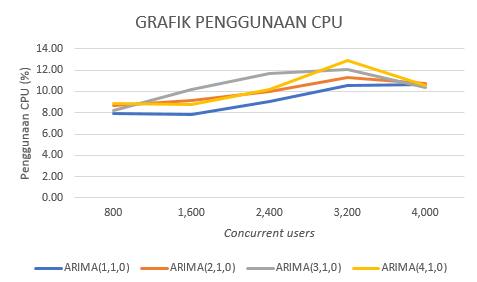
\includegraphics[width=8.7cm,height=4.7cm]{Images/C-5/cpuusage.png}
				\caption{Grafik Penggunaan CPU}
				\label{gcpuusage}
			\end{figure}
            
        \subsubsection{Penggunaan \textit{Memory}}            
            Dari hasil uji coba penggunaan \textit{memory}, semakin banyak \textit{request} yang diterima, semakin banyak \textit{memory} yang diperlukan. Perhitungan penggunaan \textit{memory} adalah rata-rata penggunaan dari masing-masing \textit{container} sebuah aplikasi. Untuk masing-masing \textit{container}, dibatasi penggunaan maksimal \textit{memory} adalah 512 MB. Dari hasil uji coba ini, dapat dilihat pada Tabel \ref{penggunaanmemory} bahwa penggunaan terbesar hanya sebesar 158.71 MB. Artinya jumlah tersebut hanya menggunakan sepertiga dari keseluruhan \textit{memory} yang bisa digunakan.
            \begin{longtable}{|p{0.22\textwidth}|p{0.10\textwidth}|p{0.10\textwidth}|p{0.10\textwidth}|p{0.10\textwidth}|p{0.10\textwidth}|}
        \caption{Penggunaan \textit{Memory}} \label{penggunaanmemory} \\
            \hline
            & \textbf{800} & \textbf{1600} & \textbf{2400} & \textbf{3200} & \textbf{4000} \\ \hline
            \endfirsthead
            \caption[]{Penggunaan \textit{Memory}} \\
            \hline
            & \textbf{800} & \textbf{1600} & \textbf{2400} & \textbf{3200} & \textbf{4000} \\ \hline
            \endhead
            \endfoot
            \endlastfoot
			
           	ARIMA(1,1,0) & 67.91 & 88.97 & 130.79 & 120.14 & 157.73 \\ \hline
            ARIMA(2,1,0) & 65.89 & 97.98 & 123.47 & 156.64 & 158.33 \\ \hline
            ARIMA(3,1,0) & 72.20 & 99.72 & 125.56 & 144.42 & 152.14 \\ \hline
            ARIMA(4,1,0) & 69.60 & 77.34 & 117.39 & 149.76 & 158.71 \\ \hline

		\end{longtable}
            
            Hasil uji coba performa penggunaan \textit{memory} dalam grafik ditunjukkan pada Gambar \ref{gmemoryusage}.
            
        	\begin{figure}[H]
				\centering
				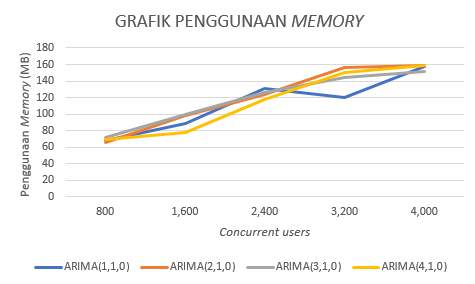
\includegraphics[width=8.7cm,height=4.7cm]{Images/C-5/memoryusage.png}
				\caption{Grafik Penggunaan Memory}
				\label{gmemoryusage}
			\end{figure}
            
        \subsubsection{Keberhasilan \textit{Request}}
        	Pada uji coba ini, dilakukan perhitungan seberapa besar jumlah \textit{request} yang gagal dilakukan. Untuk jumlah \textit{concurrent user} pada tingkat 800 dan 1600, dapat dilihat pada Table \ref{keberhasilanrequest} \textit{error} yang terjadi hampir sama. Prediksi menggunakan ARIMA(4,1,0) berhasil unggul karena menggunakan parameter yang lebih banyak. Namun hal tersebut tidak berlaku untuk ARIMA(3,1,0) karena walaupun parameternya lebih banyak dari ARIMA(2,1,0), tapi hasil prediksinya bisa meleset saat terjadi kondisi dimana koefisien negatif atau koefisien ke dua dikalikan dengan sebuah parameter bukan nol, dan koefisien lain dikalikan dengan parameter nol, maka hasil prediksinya akan negatif, yang mana seharusnya tidak mungkin ada \textit{request} negatif.
            \begin{longtable}{|p{0.22\textwidth}|p{0.10\textwidth}|p{0.10\textwidth}|p{0.10\textwidth}|p{0.10\textwidth}|p{0.10\textwidth}|}
        \caption{\textit{Error Ratio Request}} \label{keberhasilanrequest} \\
            \hline
            & \textbf{800} & \textbf{1600} & \textbf{2400} & \textbf{3200} & \textbf{4000} \\ \hline
            \endfirsthead
            \caption[]{\textit{Error Ratio Request}} \\
            \hline
            & \textbf{800} & \textbf{1600} & \textbf{2400} & \textbf{3200} & \textbf{4000} \\ \hline
            \endhead
            \endfoot
            \endlastfoot
			
            ARIMA(1,1,0) & 5.72\% & 8.96\% & 12.85\% & 12.54\% & 13.38\% \\ \hline
            ARIMA(2,1,0) & 4.31\% & 9.35\% & 10.68\% & 8.11\% & 9.04\% \\ \hline
            ARIMA(3,1,0) & 4.84\% & 10.02\% & 13.22\% & 8.63\% & 12.24\% \\ \hline
            ARIMA(4,1,0) & 4.62\% & 8.41\% & 9.39\% & 7.52\% & 9.21\% \\ \hline
		\end{longtable}
            
    		\begin{figure}[H]
				\centering
				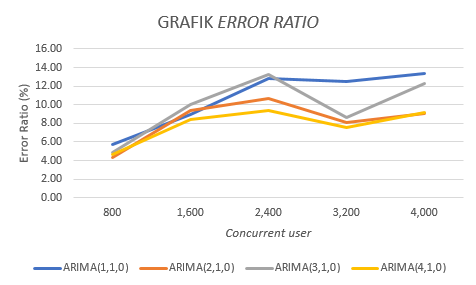
\includegraphics[width=8.7cm,height=4.4cm]{Images/C-5/errorratio.png}
				\caption{Grafik Error Ratio}
				\label{gerrorratio}
			\end{figure}
            Dari uji coba itu, 90\% lebih \textit{request} berhasil ditangani. Hasil uji coba jumlah \textit{request} yang gagal ditunjukkan dengan grafik pada Gambar \ref{gerrorratio}.